\documentclass{beamer}
\usepackage{amssymb,amsmath,amsthm}
\usepackage{graphicx}
\usepackage{tikz}
%\usefonttheme{professionalfonts}
%\usetheme{Singapore}
\usetheme{Boadilla}
\usecolortheme{rose}
\usepackage{amsmath, tikz, amsthm, amssymb}
\usepackage{hyperref}
\usetikzlibrary{matrix, tikzmark}
\usepackage{makecell} %for making \hline thicker, used in a frame with a sudoku puzzle on it!
\usepackage{array, tabularx, boldline}
\usepackage{xkeyval}
\usepackage{colortbl}
\usepackage{graphicx}
\usepackage{pdfpages}
\tikzstyle{every picture}+=[remember picture,baseline]
\tikzstyle{every node}+=[inner sep=0pt,anchor=base,
minimum width=1.5cm,align=center,text depth=.25ex,outer sep=1.5pt]
\tikzstyle{every path}+=[thick, rounded corners]

%\setframetemplate{frametitle}[default][center]

\newcommand{\macro}{}

\title{Byzantine Generals problem}
\author{Amirreza Taghizadeh}

\begin{document}
	\maketitle
	\AtBeginEnvironment{frame}{\setcounter{footnote}{0}}		%for reseting the footnote counter 
\begin{frame}

 In this presentation, we aim to discuss a problem in distributed systems known as "\textbf{Byzantine generals problem"} proposed by \textbf{Leslie Lamport.}



%\begin{tikzpicture}[remember picture,overlay]
%	\node[left] at(current 	page.east) { %for relative positioning, we use \node [left=1cm or right or below or above] 
%	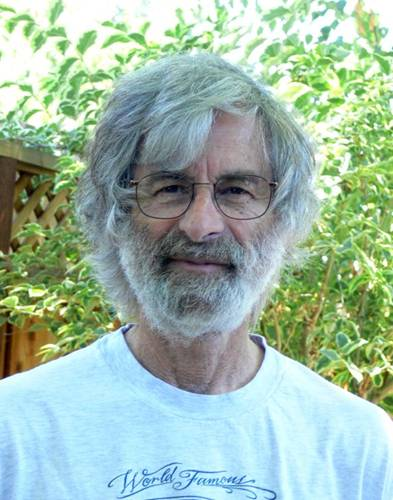
\includegraphics[width=0.4\textwidth]{lam.jpg}	
%};
%\end{tikzpicture}
\end{frame}

%%%%%%%%

\begin{frame}{Outline}
	\tableofcontents
\end{frame}
% Current section
\AtBeginSection[ ]
{
	\begin{frame}{Outline}
		\tableofcontents[currentsection]
	\end{frame}
}
\section{Brief history of Lamport's works}

\begin{frame}[label=works]
	\frametitle{Brief history of Lamport's works}
	\begin{tikzpicture}[remember picture,overlay]
		\node [below= 1.9cm, left=0.8cm] at(current page.north east) { %for relative positioning, we use \node [left=1cm or right or below or above] 
			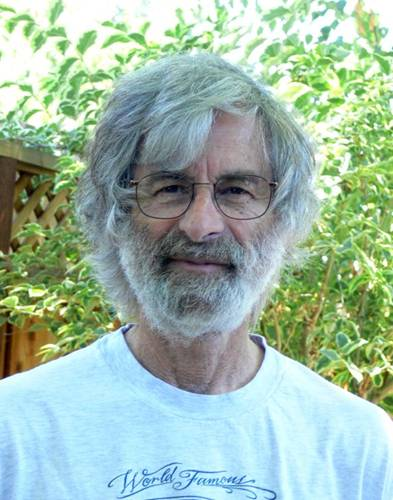
\includegraphics[width=0.24\textwidth]{lam.jpg}	
		};
	\end{tikzpicture}
	\begin{itemize}
		\item<1-> \textbf{Inventing \LaTeX: }\small a group of macros, which can make the life of \TeX users a lot easier!!
		\item<1-> \textbf{One way authentication} in Whitfield Diffie's "\textit{New directions in cryptography"} (1976)
	\end{itemize}
\end{frame}

%%%%%%%%%

\begin{frame}{brief description of \textbf{One-way Function}}
	\begin{itemize}
		\item<1-> A one way function \pmb{$f$} is a function that is \textbf{easy to compute } but whose \textbf{inverse is difficult to compute}: 
		\item<2-> or to say $f$ is one-way function iff (adapted from\footnotemark):
		\begin{enumerate}
			\item<3-> for all value $v$, finding data object $d$ s.t. $\phi(d)=v$ is \textbf{computationally infeasible.}
			\item<4-> $f$ is not \textbf{one-to-one} or proving it otherwise is \textbf{computationally infeasible.}\footnotemark 
		\end{enumerate}
	\end{itemize}
	\uncover<5->{ \centering 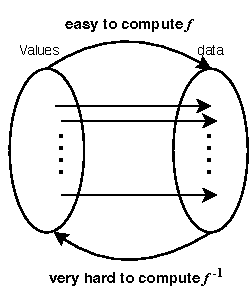
\includegraphics[width=0.3\textwidth]{myfig1.pdf}}
\footnotetext[1]{\footnotesize Lamport, "\textit{Constructing Digital Signatures from a One Way	Function}"}
\footnotetext[2]{\footnotesize i.e. to say: $\forall$ data object $d' \ne d: \phi(d') \ne \phi(d)$}
\end{frame}

%%%%%%%%%

\begin{frame}{brief description of \textbf{One-way Authentication}}
	\begin{definition}[Digital signature]
		A digital signature created by \textbf{sender P} for \textbf{document m} is a data item $\sigma_p (m)$ that is when received together with \textbf{m}, one can determine (e.g. in a court of law) that \textbf{P} generated document \textbf{m}.\\
		\uncover<2->{Hence A tool for determining \textbf{validity} of something sent.\footnotemark}
	\end{definition}

\footnotetext[1]{\footnotesize Lamport, L. (1979) "\textit{Constructing Digital Signatures from a One Way	Function}"}
\end{frame}

%%%%%%%%%

\begin{frame}{brief description of \textbf{One-way Authentication}}
	\begin{definition}[One way authentication]
		It must be \textbf{easy for anyone} to recognize the signature as \textbf{authentic} but \textbf{impossible} for anyone other than the signer to produce it!\footnotemark
	\end{definition}
\footnotetext[1]{\footnotesize Diffie, W. (1976)"\textit{New Directions in Cryptography}"}
\end{frame}

%%%%%%%%%%%%

\begin{frame}{A practical Example of a \textbf{One-way function} in \textbf{one-way authentication} \\ \ \textbf{Login Problem}}
	\begin{itemize}
		\item<1-> User \textbf{A} enters Password \textbf{$PW$} and computer store it as \textbf{$f(PW)$} 
		\item<2-> where $f(PW)$ is a one-way function of \underline{10 million instructions}
		\item <3-> and its inverse has $10^{30}$ more instructions (or computations), which practically makes it \textbf{noninvertible}
		\item <4-> for example, finding square root of $x_0$ given in $f(x)=x^2$ is much harder than computing $x^2$ at $x_0$.
	\end{itemize}
\end{frame}

%%%%%%%%

\begin{frame}{brief description of \textbf{One-way Authentication} \textit{Cont'd}}
	\begin{itemize}
	\item <1-1>However, determining exactly what the one-way function should be is originally solved by \textbf{Lamport} \\ which further lead to the publication of the paper: "\textit{Constructing Digital Signatures from a One Way Function}"
	\item<2-> But how this solution relates to the ecosystem of \textbf{public keys} is \underline {out of the scope of the presentation} and discussed in the paper:\\ \textit{"New Directions in Cryptography"} by Whitfield Diffie (1976) 
\end{itemize}
\end{frame}

%%%%%%%%%%%%%
\begin{frame}[label=works]
	\frametitle{Brief history of Lamport's works}
	\begin{itemize}
		\item<1-> \textbf{Inventing \LaTeX: }\small a group of macros, which can make the life of \TeX users a lot easier!!
		\item<1-> \textbf{One way authentication} in Whitfield Diffie's "\textit{New directions in cryptography"} (1976)
		\item <1-> \textbf{bakery algorithm} an algorithm to ensure mutual exclusion in concurrent processes
		\item <2->  that is to ensure a data structure is modified by at most one process at a time
		\\ and no process is reading a data structure while it is being written by other processes. 
		\item <3-> \textbf {Paxos algorithm}: an algorithm used in distributed systems for reaching consensus, used in distributed storage systems
	\end{itemize}
\footnotetext[1]{Silberschatz, "Database System Concepts", Ch. 19, P. 965}
\end{frame}
%%%%%%%%%%%%%

\begin{frame}
	\frametitle{Brief history of Lamport's works \textit{cont'd}}
	\begin{itemize}
		\item <1-> Time, clocks and ordering of events in a distributed system:
		\begin{itemize}
			\item<2-> \footnotesize in a distributed system, sometimes it is \textbf{impossible} to say an event has happened before something else. 
			\item <3-7> \footnotesize hence, relation "\textit{happened before} is a partial ordering relation.
			\item <4-5> \textbf{Partial ordering? sounds familiar...}
			\alt<5> {\begin{definition} [Partial ordering]
				Partial ordering relation is an ordering relation in which not all members of the set need to be comparable!
			\end{definition}}{}
		\item <6-> \footnotesize He proposed in that paper a partial ordering of "happened before" and gave a \textbf{distributed algorithm} for \textbf{extending it to a total ordering of events}
		\newline \newline
		
		\end{itemize}
	\end{itemize}
\uncover<7-> {\centering \large \textbf{But where is the "Byzantine generals" problem in the list?}}
%\only{hi}<6>
\end{frame}

%%%%%%%%%

\section{Origination of Bezyntine Generals problem}
\begin{frame}
	\frametitle{Brief history of the origination of the problem}
	\begin{itemize}
		\item<1-> \textbf{Naming:} "As the Edsger W. Dijkstra's {"Dining philosophers \textit(a classic problem discussed in Operating Systems classes) involves a story, I decided to \textbf{include a story with the problem} related to Digital signatures with a recursive solution algorithm"} -Lamport
		\item<2-> \textbf{Motivation:} Two General's problem. \uncover<3->{in fact, byzantine generals are a more general form of this problem.}
	\end{itemize}
\end{frame}

%%%%%%%%%%%

\begin{frame}
	\frametitle{A brief Overview of Two general's problem}
	\framesubtitle {\large Stating the problem through visualization!}
\begin{tikzpicture}[remember picture,overlay]
	\node[above=1cm] at(current 	page.south) { %for relative positioning, we use \node [left=1cm or right or below or above] 
		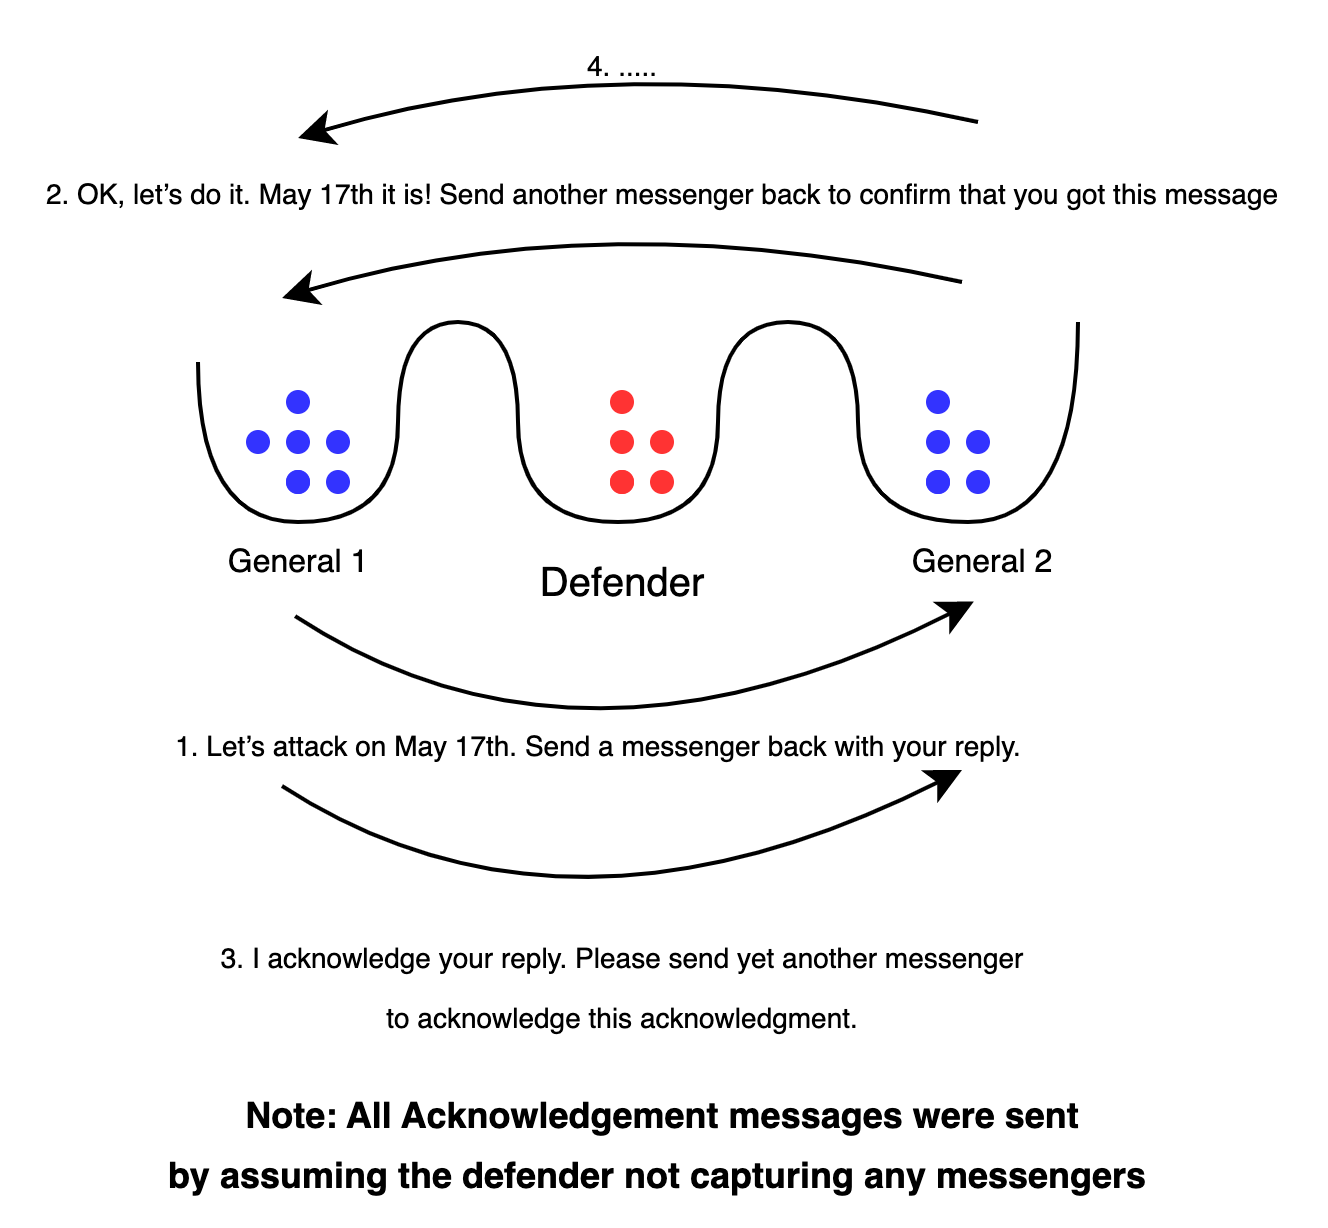
\includegraphics[width=0.6\textwidth]{myfig2.png}	
	};
\end{tikzpicture}
\end{frame}

%%%%%%%%%%%%%%%


\section{A review of the Byzantine problem}
\begin{frame}{A review of the Byzantine problem}
	\begin{itemize}
		\item <1-> There is an \textbf{enemy city} and a group of \textbf{General $i$}, each deciding to reach \textbf{an agreed upon plant} (which is the exact definition of \textbf{consensus})
		\item <2-> and each general $i$ is equipped with a messaging method for sending value $v(i)$
		\item <3-> AND there are a \large bunch of \textbf{traitorous generals} \normalsize sending \textbf{conflicting} messages, aim to prevent \textbf{loyal generals to reach a plan}
		\item <4-> In order for them to a reach consensus, two conditions must be satisfied:
		\begin{enumerate}
			\item <5-> Every loyal general must obtain the same information $v(1), v(2) \dots, v(n)$
			\item <5-> The value sent by a loyal general should be used by all loyal generals
		\end{enumerate}
	\end{itemize} 
\end{frame}

%%%%%%%%%%%%%%%%%%

\begin{frame}{A review of the Byzantine problem \textit{cont}}
	\uncover <1->{How should the generals send their messages?\newline}
	\uncover<2-> {Let's examine how \textbf{a single general $i$ should send the message $v(i)$} that is formally defined by:}
	\uncover<3->{\small(which is made by grouping generals into two groups, namely \textbf{commander and lieutenant generals})}
	\uncover <3->{\begin{definition} [Byzantine Generals Problem]
		A \textbf{commanding general} must send an order to his \textbf{$n-1$ lieutenant generals} s.t.:\newline
		IC1. All loyal lieutenants obey the same order.\newline
		IC2. If the commanding general is loyal, then every loyal lieutenant obeys the order he sends.
	\end{definition}}
\uncover<4->{\small Note that IC2 $\implies$ IC1}
\end{frame}

%%%%%%%%%%%%

\begin{frame}{A review of the Byzantine problem \textit{cont}}
	\uncover<1->{Lamport gave a recursive algorithm based on \textbf{majority function} for the mentioned problem in case of having \textbf{oral messages} whose content is solely managed by the sender.}
	\uncover<2->{\newline \newline Unfortunately, the algorithm works only, in case of having $m$ traitors, for $n\ge 3m+1$ generals}
	\newline \newline
	\uncover<3->{\begin{center}
			\Large This is where he proposed an algorithm based on \textbf{unforgeable messages.}
		\end{center}}
\end{frame}

%%%%%%%%%%%%

\section{Signed messages}
\begin{frame}{Signed messages}
	\uncover <1->{\Large What was wrong with the oral messages??\newline}
	\uncover<2->{\normalsize Answer: because \textbf{traitors lie}, they \textbf{alter the contents} of the messages they receive and send \newline}
	\uncover<3>{\begin{tikzpicture}[remember picture,overlay]
			\node at(current 	page.south) { %for relative positioning, we use \node [left=1cm or right or below or above] 
				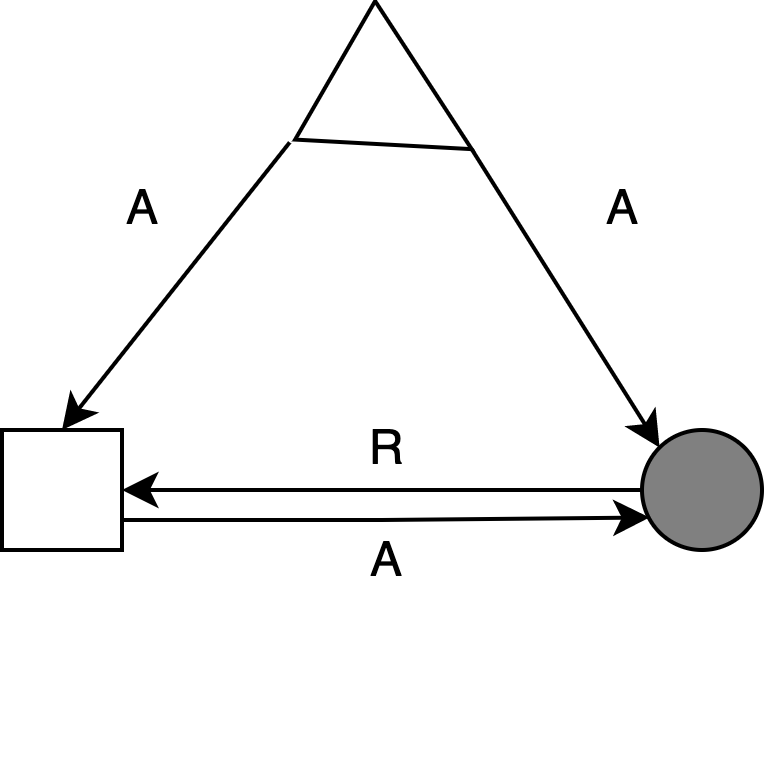
\includegraphics[width=0.4\textwidth]{fig1.png}	
			};
	\end{tikzpicture}}
\uncover<4>{Let's make messages that can not be lied (forged) or any alterations could be detected}
\end{frame}

%%%%%%%%%%%%%

\begin{frame}{Signed messages algorithm}
	\uncover<1>{Note that we know  \textbf{the number of m} traitors when running the Alg.}
	\begin{enumerate}
		\item<2-> Commander sends a message having a value $v$ and a signature (which is a sequence of IDs) $\rightarrow \pmb{v:0}$
		 \item<3-> each lieutenant $i$ receives the message of length $k$, \\ \textbf{adds the $v$ to a $V_i$ set}, \textbf{adds his ID} to the message and \textbf{sends it to those child lieutenants not having received this message before}
		 \item <4-> when lieutenant $i$ receives no more messages, the lieutenant $i$ applies the \textbf{a Choice function} to $V_i$ in order to retrieve an order.
	\end{enumerate}
\uncover<5>{what is that \textbf{Choice function?}}	
\end{frame}

%%%%%%%%%%%%%%%%%

\begin{frame}{Choice function}
	The Choice function could be any \textbf{aggregate function} (such as median, average, etc) \large BUT, \normalsize it needs to have two essential properties:
	\begin{enumerate}
		\item <1-> if Set $V_i$ consists of single value $v$ Then, $Choice(V_i)={v}$
		\item<2-> $Choice(\emptyset) = RETREAT$ 
	\end{enumerate} 
\end{frame}

%%%%%%%%%%%%%
%%we should use [fragile] for using verbatim environment
\begin{frame}[fragile]{Formal statement of Signed messages }
Initially $V_i=\emptyset$\\
(1) The commander signs and sends message $v:0$ to all lieutenants\\
(2) For each $i$:\\
\quad(A) If Lieutenant $i$ receives a message of the form $v:0$ from the commander and he hasn't receieved any order, then:\\
\quad \quad(i) he lets $V_i={v}$\\ 
\quad \quad (ii) he sends the message $v:0:i$ to every other lieutenant.\newline \newline
\quad (B) If Lieutenant $i$ receives a message of the form $v:0:j_1\dots:j_k$ \textbf{and} $v\notin V_i$ then:\\
\quad \quad(i) he adds $v$ to $V_i$;\\
\quad \quad (ii) if $k<m$, then he sends the message $v:0:j_1\dots:j_k:i$ to every lieutenant other than $j_1,\dots,j_k$\newline \newline
(3) For each $i$: When Lieutenant i will receive no more messages, he obeys the order $Choice(V_i)$
\end{frame}

%%%%%%%%%%%%

\begin{frame}{The impossible case revisited}
	\begin{tikzpicture}[remember picture,overlay]
		\node at(current 	page.south) { %for relative positioning, we use \node [left=1cm or right or below or above] 
			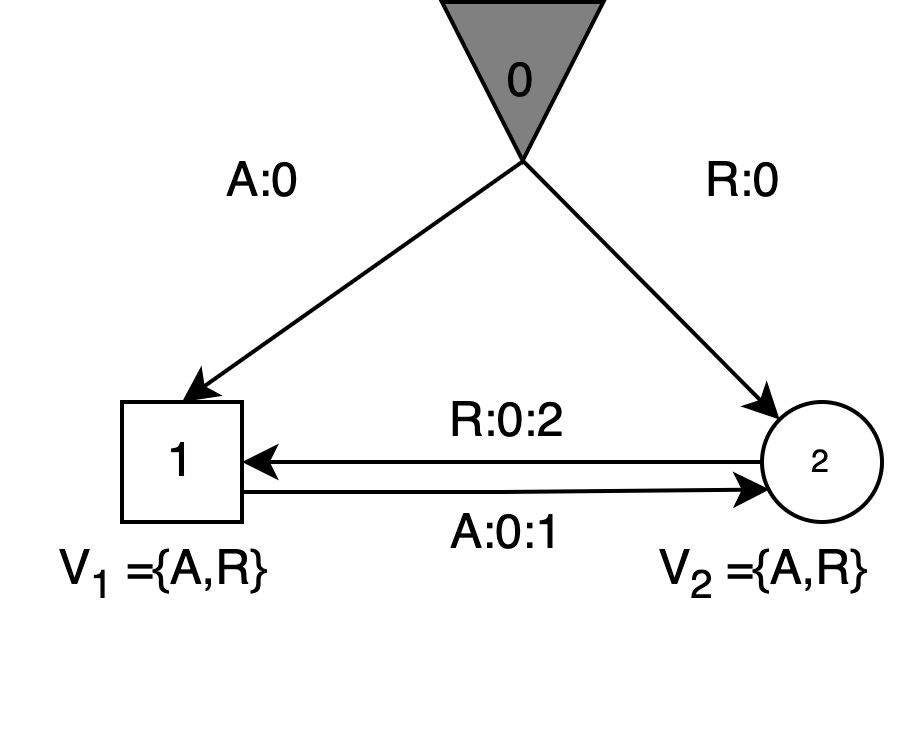
\includegraphics[width=0.8\textwidth]{fig3.png}	
		};
	\end{tikzpicture}
\end{frame}


\section{Solving consensus in asynchronous and synchronous systems}
\begin{frame}
	Through the end of the presentation, we will be talking about \textbf{Consensus in asynchronous} systems \\ and an important Article in this regard, by Fischer-Lynch-Paterson (FLP) \\ Which proves the impossibility of \textbf{reaching consensus} in \textbf{asynchronous system} in the presence of any failure.
	\\ However, in the paper 
\end{frame}
\begin{frame}{Asynchronous systems $\rightarrow$ Lamport's Time clocks revisted}
	\small
\begin{definition}[Asynchronous system\footnotemark]
	In such systems, there is no time assumptions about processes. That is, we do not have \textbf{physical clock}. Instead \textbf{Time} is defined with respect to communication and measured by a \textit{Logical clock}.  
\end{definition}
\uncover <2-> {Here is Lamport's Algorithm for finding something has "happened before" something else.}
\footnotetext[1]{\textit{"Reliable and Secure Distributed Programming"} A book by Rodrigues L. \& Cachin C. }
\end{frame}

%%%%%%%%%%%%%
\begin{frame}{Lamport's Algorithm for Time clocks}
\begin{enumerate}
	\item <1-> Each process $p$ keeps an ineger called \textit{logical clock $l_p$} initially 0.
	\item <2-> Whenver an event occurs at Node $p$, the logical clock $l_p$ is incremented by one unit.
	\item <3-> When a process \textbf{sends a message,} it adds a timestamp to the message with the value of its logical clock at the moment the message is sent. The timestamp of an event $e$ is denoted by $t(e)$.
	\item<4-> When a Node $p$ receives a message $m$ with timestamp $t_m$, Node $p$ increments its logical clock in the following way: $l_p := \max\{l_p, t_m\} + 1$
\end{enumerate}
	\footnotetext[1]{\textit{"Reliable and Secure Distributed Programming"} A book by Rodrigues L. \& Cachin C. }
\end{frame}

\end{document}